\chapter{Android}
\label{ch:Android}

\author{Nico Leidenfrost}
%
Android is a linux distribution and is currently developed by the software giant Google. Android is an operating system with primary focus on mobile devices with a built-in touchscreen. The most popular examples, in which Android is used, would be smartphones and tablets. Since Android is an open source project, developers all over the world can contribute to it and even build their own Android system. Android programs are called ``apps'' which is the short version of application, these applications extend the basic functionality of an Android device.

\section{History of Android}
Android started as a startup Company under the name ``Android Inc.'', founded in October 2003, in the US city Palo Alto, California. At first its purpose was to serve as an operating system for digital cameras, that would be more advanced than the standard in 2003. One Year later in 2004 they changed their goals to focus on mobile phones instead of cameras because the market declined their approach. Google became aware of this company and acquired it in July 2005 along with its founding members. The first working prototype of an Android smartphone looked quite similar to a BlackBerry phone of the time, because it had the BlackBerry typical QWERTY keyboard. They made two versions of this prototype, both without a touchscreen. In 2007, Apple introduced the iPhone which already featured a touchscreen. Since then Google also focused on mobile devices that included a touchscreen, but also stated that a touchscreen could never fully replace physical buttons. The first officially sold Android smartphone that was the HTC Dream, launched in 2008. Google continued to maintain the Android project and launched many updates which introduced new features or just fixed existing bugs. The developers of Android did choose a quite funny naming scheme for their major releases, namely the names of desserts. Each version starting with ongoing letters from the alphabet starting with ``Cupcake'' as the name for version 1.5. After that came version 1.6 called ``Donut'' up to 7.0 as ``Nougat'' and the latest version 8.0 as ``Oreo''. Google explained this naming scheme with the statement, ``Since these devices make our lives so sweet, each Android version is named after a dessert''.

\section{Design}
Material Design is Google's visual design language that was first introduced in 2014. The goal was to develop a single underlying system that allows for a unified experience across all kinds of devices. It tries to support visual elements with the characteristics of real materials, hence Material Design. These guidelines help the users to interact and quickly understand different kinds of User Interface (UI) elements by using familiar tactile attributes.

GRAMOC's Android app uses these design principles for the user interface as shown in figure \ref{fig:appscreenshots}

\begin{figure}[H]
    \centering
    \begin{tabular}{cc}
    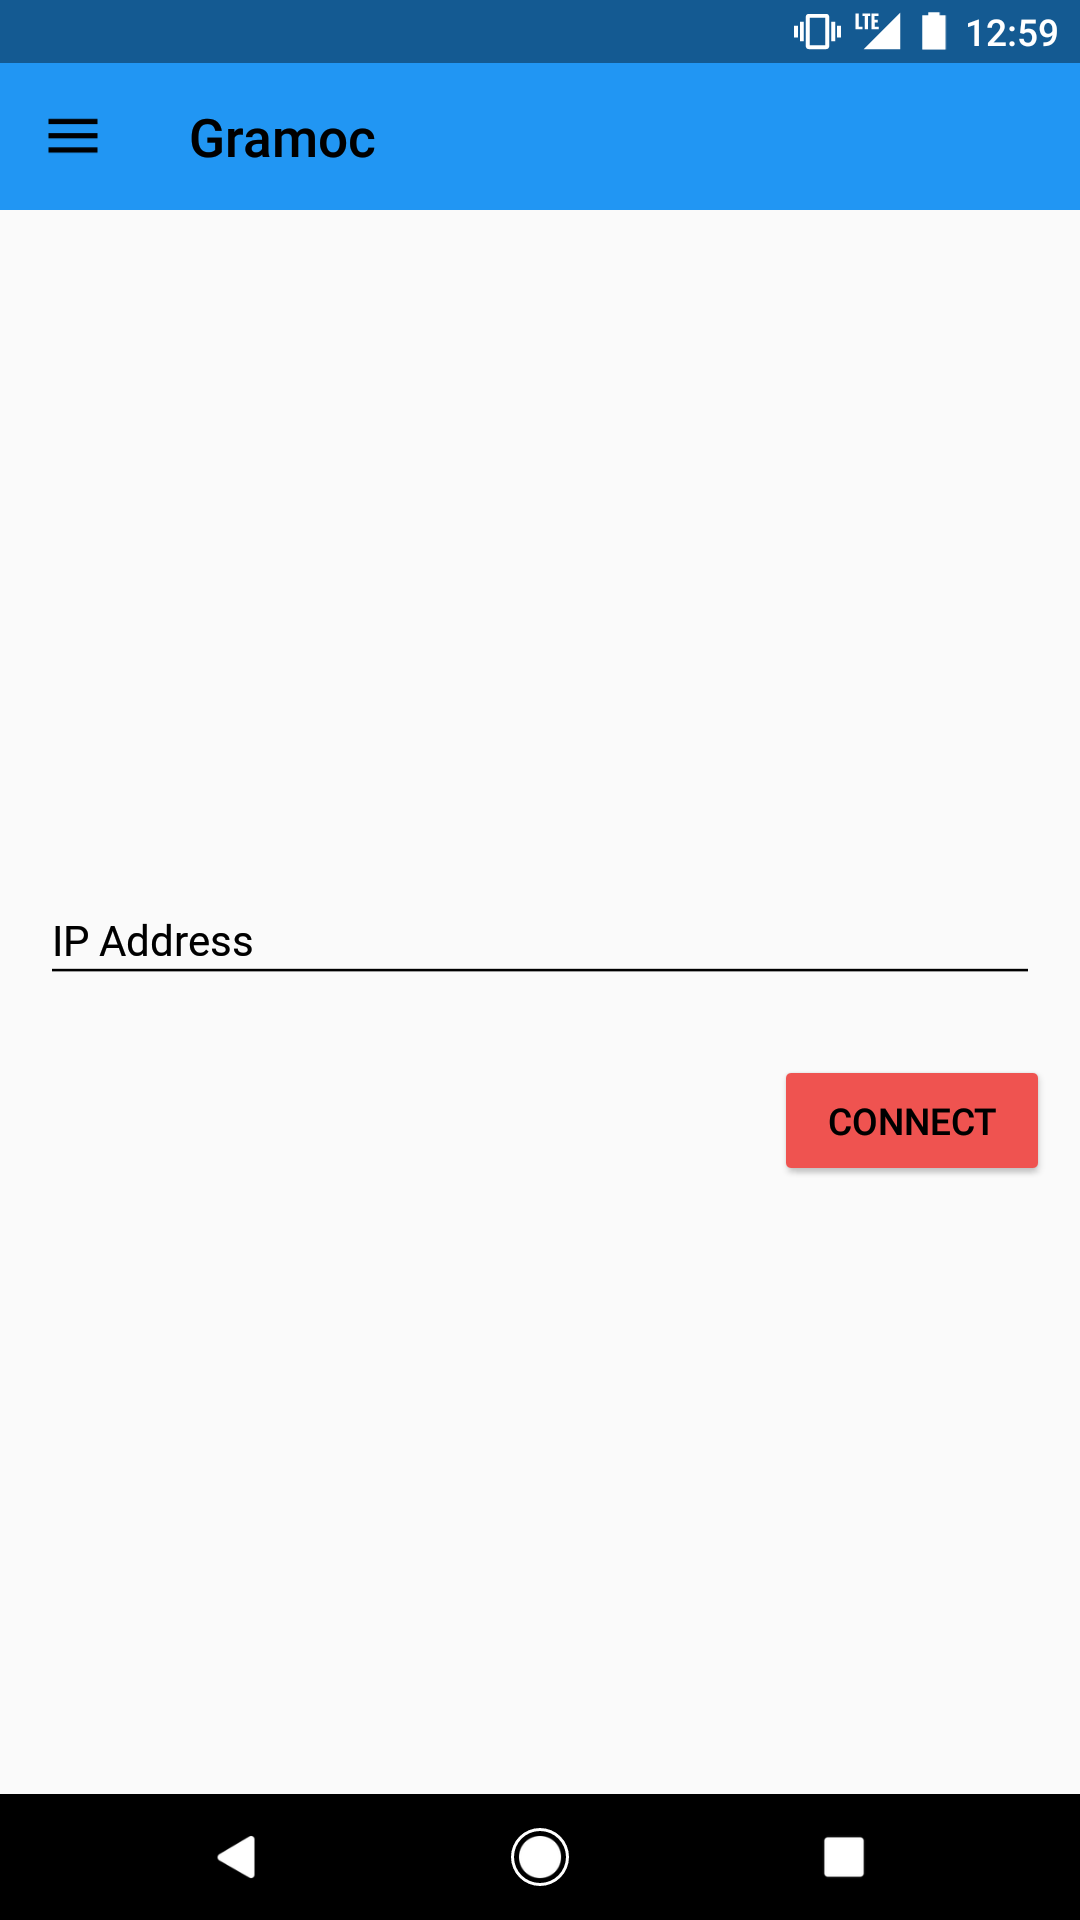
\includegraphics[height=7cm,keepaspectratio]{app_connect}
    &
    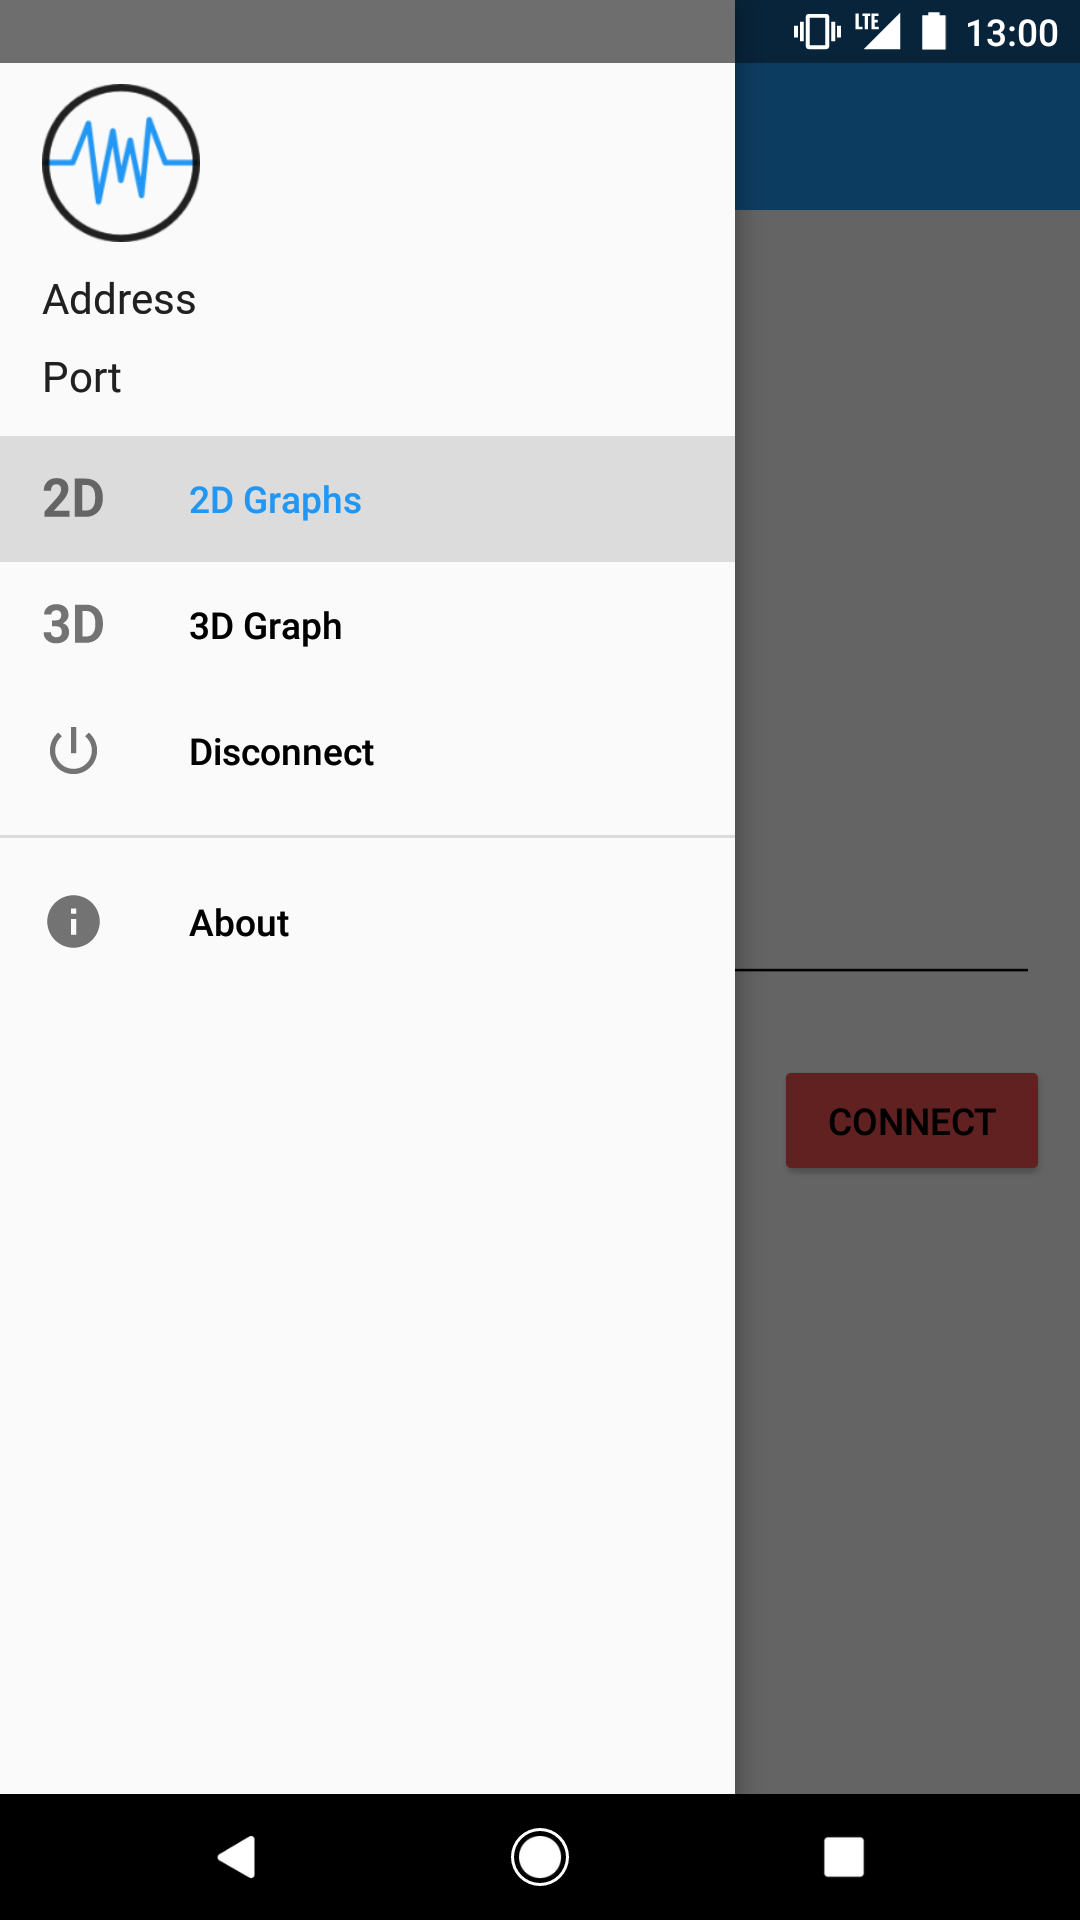
\includegraphics[height=7cm,keepaspectratio]{app_navdrawer}
    \\
    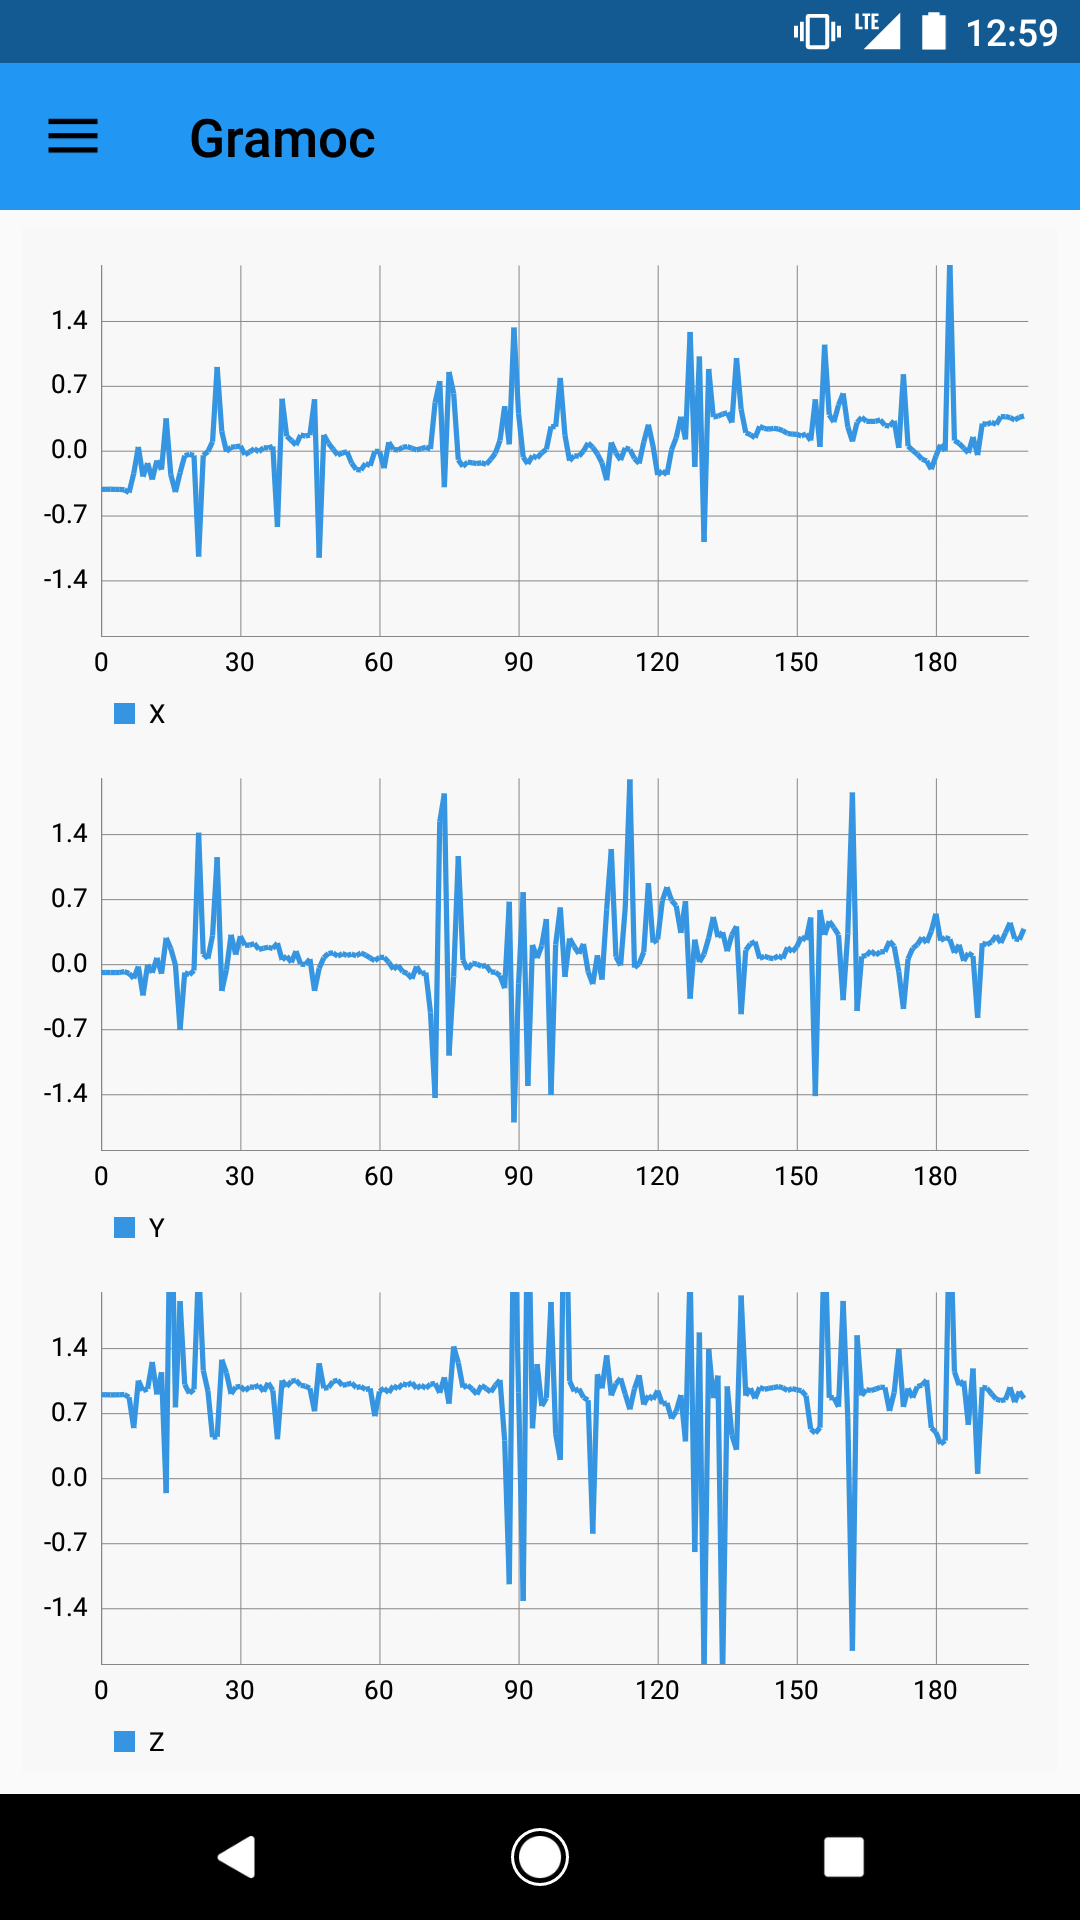
\includegraphics[height=7cm,keepaspectratio]{app_sensor}
    &
    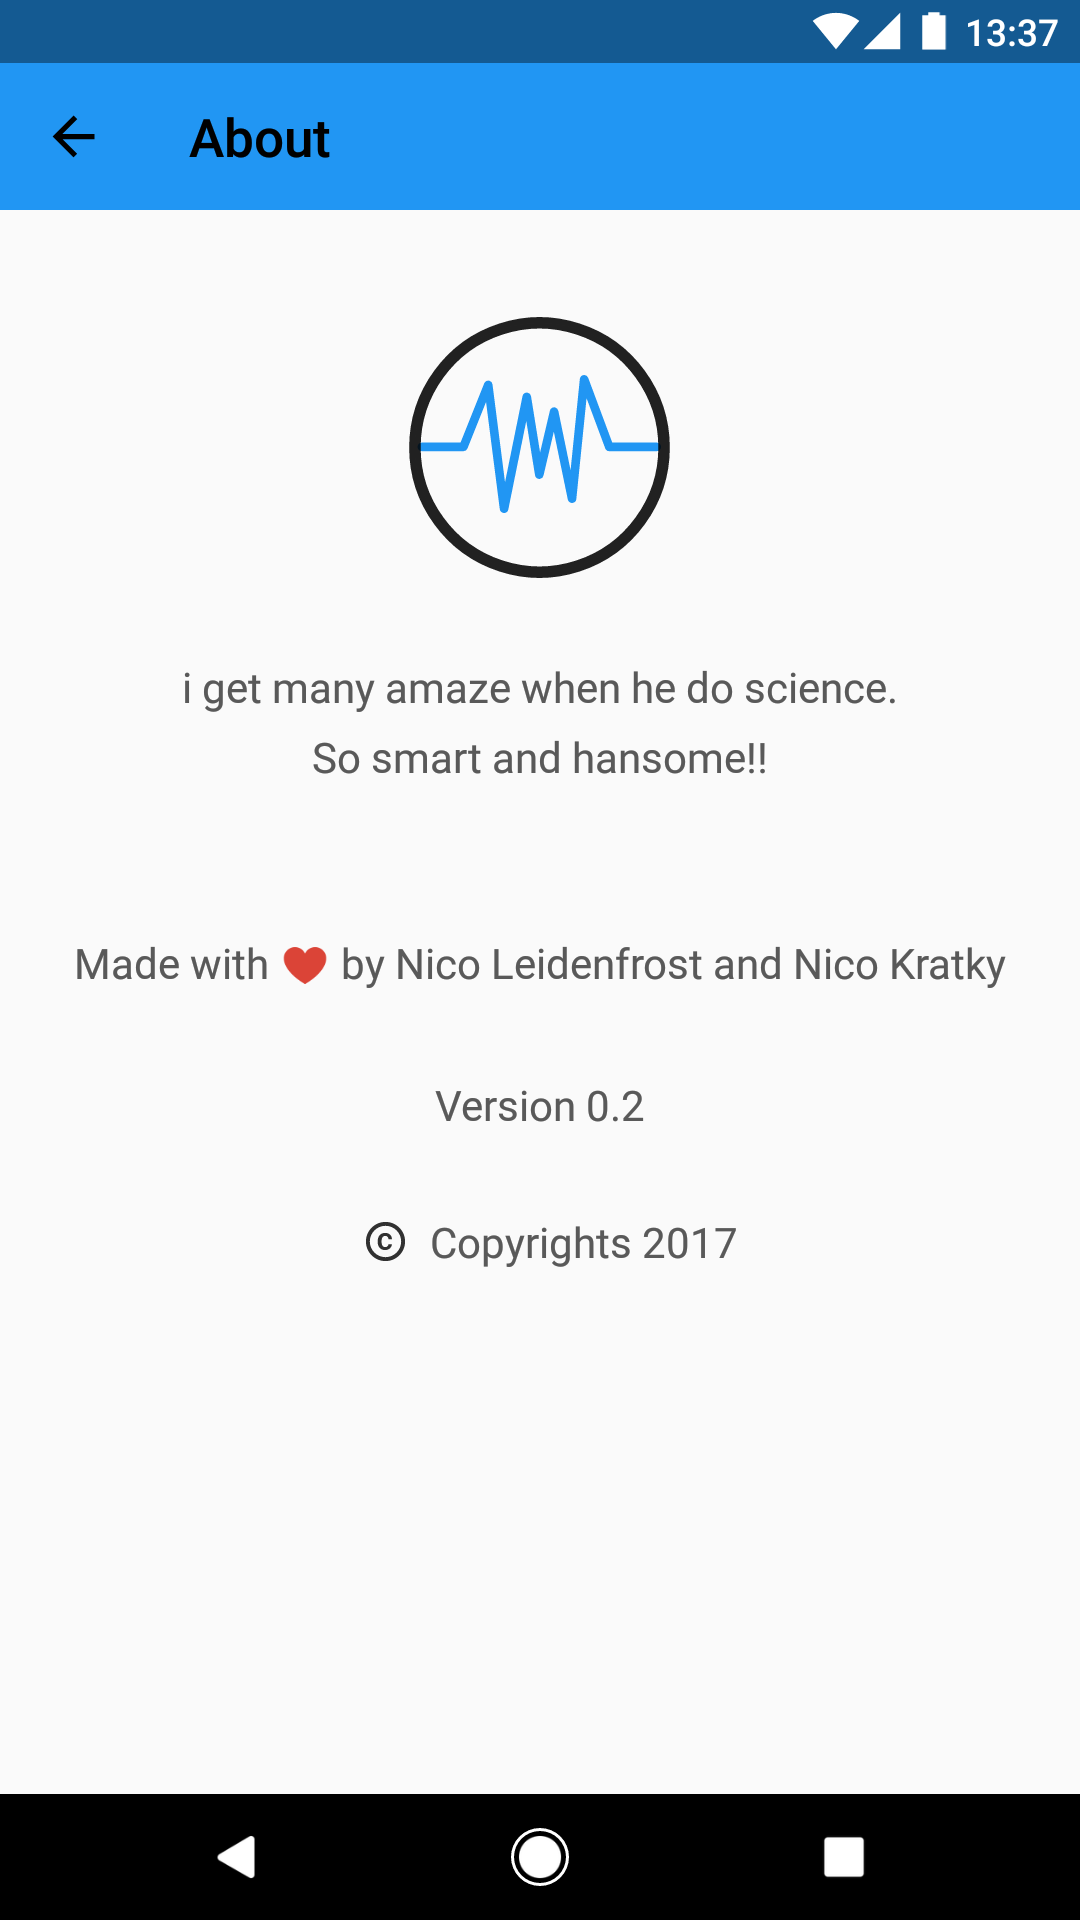
\includegraphics[height=7cm,keepaspectratio]{app_about}
    \end{tabular}
    \caption{Screenshots of App}
    \label{fig:appscreenshots}
\end{figure}

\section{Overview of Android Application Development}
Applications are often abbreviated as ``apps''. To write Android apps one must use the Android software development kit (SDK). The variety of programming languages that can be used is not very broad so a developer must choose one of a few options to build a native Android app.

\subsection{Java}
Java is the programming language used by the most people to develop an Android application. The majority of apps and libraries are written in Java. These apps are compiled to bytecode which then will be translated to native instruction by the Android Runtime (ART). ART is an application runtime environment that replaced its predecessor Dalvik, a process virtual machine developed to run Android applications. Java was the programming language chosen to build the Android application in this project because of the broad variety of third-party libraries and support available.

\subsection{C/C++}
With C or C++ code and the Android native development kit (NDK), a native library for Android, applications can get much better results in terms of performance. The reason behind this is that the C/C++ code does not need a virtual machine to be executed (i.e. the code runs natively), therefore the performance of an application that uses C or C++ code can be much higher than the performance of an app written only in Java. Important is to mention that an Android application should not be written entirely in C/C++ because all the UI still needs to be handled by the Android framework and thats only available in Java. Since the Java native interface (JNI) handles the interoperability of the two languages and also adds a lot of complexity to the application it would be best to only write functions that require a high CPU performance in C or C++ code.

\subsection{Go}
``The Go programming language is an open source project developed by a team at Google and many contributers from the open source community'' \autocite{GoProject}. This programming language is supported although there are limitations to the application programming interfaces (API), therefore it was not considered a reasonable option for GRAMOC.

\subsection{Kotlin}
Kotlin is a modern and powerful language, which is officially supported since May 2017 and solved various issues addressed with Java (e.g. Null references). Kotlin is interoperable with Java which means an Android application can contain both Kotlin and Java code. Kotlin was considered to be used in this project but the fact that the official support was only recently introduced and therefore the amount of available third-party libraries is not as comprehensive as in Java, led to the decision that Java was the programming language of choice.

\subsection{Runtime}
A runtime refers to a system that converts code implemented in a high level language like Java into CPU readable byte code. Compiled Java code can not run on any machine because the code is compiled to Java byte code, which a CPU can not interpret. To run this Java byte code, the Java virtual machine (JVM) is needed, because it translates the Java byte code into CPU readable byte code. In Android however the Java code is compiled to Java byte code, then compiled again to Dalvik byte code and then given to the runtime. Two different types of a runtime were introduced in Android.

    \subsubsection{Dalvik}
    The Dalvik Virtual Machine (DVM) was the first runtime used in Android. The DVM was chosen instead of the JVM to be used in the early days of Android because it could perform better when running multiple apps at once. Both virtual machines are quite similar to each other, except the matter that the JVM is stack-based and the DVM is register based, which means the DVM needs less instructions, but these must be more complex. At first Android devices only had a small amount of memory available, therefore the just-in-time (JIT) compilation of the DVM was a perfect concept because it resulted in a small memory footprint. This was achieved by only translating and caching the chunks of byte code that were needed to execute the next few steps of an application. So instead of compiling the whole code of an application, only the parts needed were compiled.

    \subsubsection{Android Runtime Environment}
    The problem of having to few memory available was solved by the fact that the hardware improved over the years. The primary focus of application developers changed from most efficient way to use memory to improve performance and simultaneously decrease battery usage. With that in mind the Android Runtime Environment (ART), which now uses Ahead-of-Time (AOT) compilation, was created. First introduced in Android 4.4 and later replaced Dalvik completely in version 5.0, ART increased the performance of Android application by compiling the whole code at once at the time of the installation of the app. This method improved startup time, battery consumption and overall performance, because now the code does not need to be compiled during runtime.

\section{Components}
In order to build this Android application following Android components were used:

\begin{itemize}
    \item Intent
    \item Toolbar
    \item Activity
    \item Service
    \item NavigationDrawer
    \item Threads
\end{itemize}

\subsection{Intent}
``An intent is an abstract description of an operation to be performed'' \autocite{AndroidIntent}. It handles the execution of a specific action that it takes along with data to operate on. It is most used when launching a new activity.

\subsection{Toolbar}
This component is a widget from the Android \emph{appcompat support library} and is persistent throughout the whole application. Most of the time it is referred to as app bar or action bar. Since this element is persistent, it will be used to perform important actions, like searching or navigating, but also to create space for identification of an application.

\subsection{Activity}
``An activity is a single, focused thing that the user can do.'' \autocite{AndroidActivity} Each application starts with launching an activity, therefore an activity handles the creation of a new window and loads all the User Interface (UI) elements. Activities are usually shown as a full-screen window, but also as a floating window or even be embedded inside of another activity by implementing an ActivityGroup. Inside the Android-system, activities are handled as a stack, this means every time a new activity is launched, the Android system puts that activity on the top of the stack and this activity becomes the running activity. The other activities in the stack are placed below the active activity and therefore remain inactive. An activity's lifecycle can be understood as depicted in Figure \ref{fig:activitylifecycle}.

\begin{figure}[H]
    \centering
    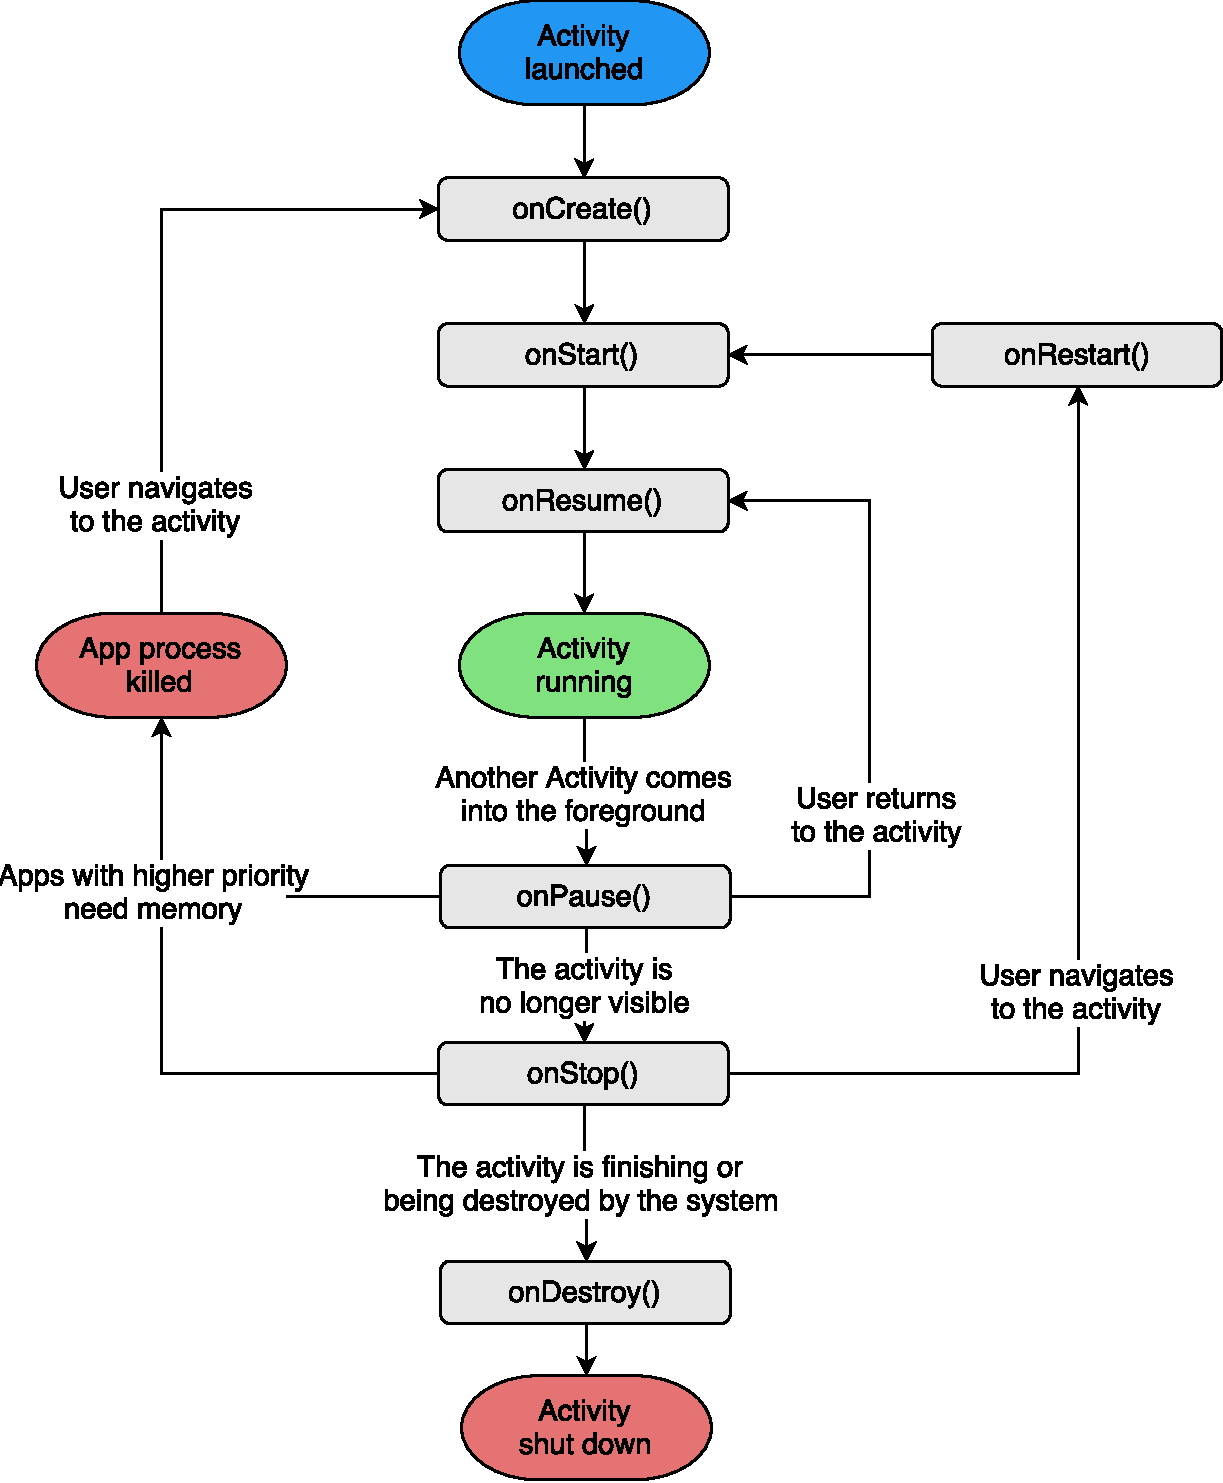
\includegraphics[width=10cm,keepaspectratio]{android-activity-lifecycle}
    \caption{Flowchart showing the lifecycle of an Android-activity}
    \label{fig:activitylifecycle}
\end{figure}

\subsection{Service}
A service is used to execute tasks in the background, which usually run a long time that do not need a visual interface to interact with an user like an activity. Once started, a service can persist in the background and is therefore not interrupted by switching applications. If another component binds itself to the service, it enables the possibility of interprocess communication (IPC). A common use case of a service is to handle network connections through it. The lifecycle is defined as depicted in Figure \ref{fig:servicelifecycle}.

\begin{figure}[H]
    \centering
    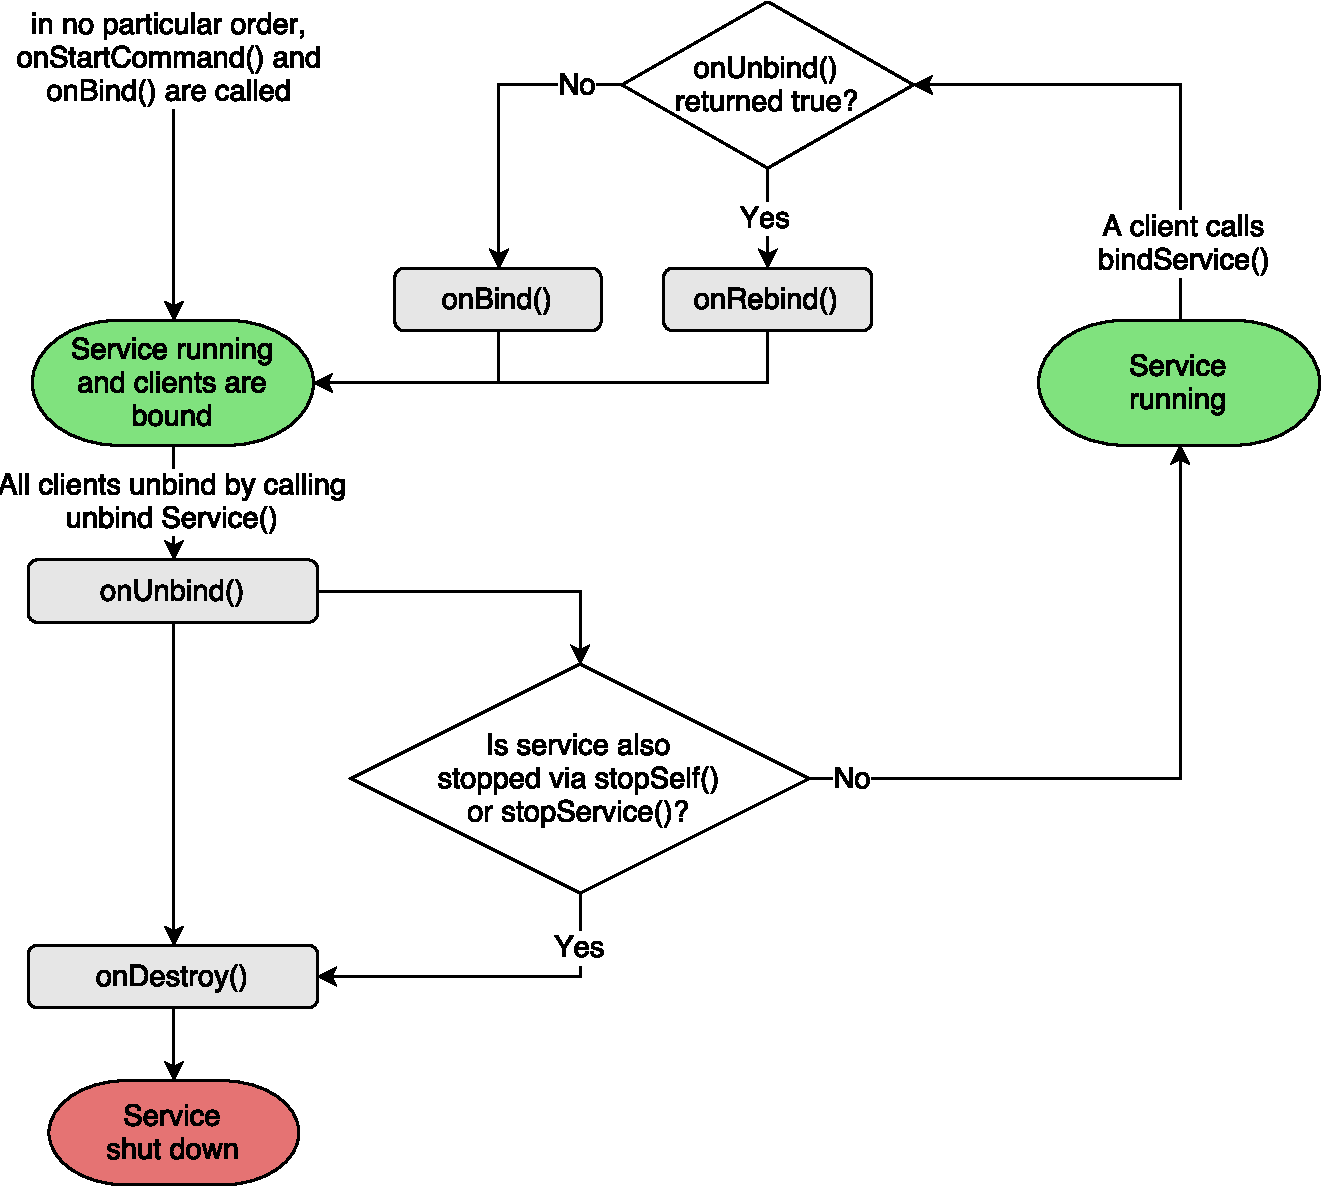
\includegraphics[width=10cm,keepaspectratio]{android-service-lifecycle}
    \caption{Flowchart showing the lifecycle of an Android-service}
    \label{fig:servicelifecycle}
\end{figure}

\subsection{NavigationDrawer}
To navigate between the activities and views a navigation drawer was implemented. A navigation drawer this is a panel which is pulled from the left border of the screen to approximately 3 quarters of the screen width and contains a header where general information is displayed and a body which contains different navigation items. The navigation drawer is included in the material design pattern, which is often used in Android application development, so most Android apps provide a navigation drawer.

\subsection{Threads}
When an Android application component is launched and it is the first component of an application Android will start a new Linux process. If this application is already running inside a process and a new component is launched or an action is preformed, Android will execute this task in the main-thread of the application unless it is explicitly stated to execute the operation in a new thread within this process. When working with threads in Android two essential rules must be followed \autocite{AndroidThreads} :

\begin{enumerate}
    \item Do not block the UI thread
    \item Do not access the Android UI toolkit from outside the UI thread
\end{enumerate}

\noindent The reasons behind this two rules are quite simple. The point why the thread that contains the user interface should never be blocked is simply because then no events could be dispatched, including events that update the UI itself. This would mean the application could not give any information to the user unless the operation which is blocking the thread has finished and thats really bad, because the user could think that the application stopped working. Accessing the UI toolkit from a thread other than the UI thread is also a bad idea, since the UI toolkit is not thread-safe. This means if multiple thread would access UI elements, a race condition could happen and therefore cause errors within the application. To avoid such errors Android implemented different ways how to execute tasks asynchronously in Android:

    \subsubsection{Extended Threads}
    The first way is to implement a subclass of the Java \emph{Thread} class. If this solution is chosen a developer must override the \emph{run} method of the superclass. If the way of how a thread handles certain situations needs to be changed or new functionalities needs to be added, a developer should choose this method, otherwise the Runnable interface should be implemented.

    \subsubsection{Runnable interface}
    Another method to accomplish asynchronous behavior would be to implement the \emph{Runnable} interface when creating a class. To execute the tasks, an instance of this class needs to be given to the thread which should execute the tasks. This way is preferred to use when running tasks which does not need modified thread behavior. When tasks from a runnable class are executed there is no need to launch a new thread for each task, instead they can be executed on various threads.

    \subsubsection{AsyncTasks}
    AsyncTasks are implemented to move work to the background and then update the UI accordingly. An AsyncTask is defined to execute blocking operations, therefore there will be only one active AsyncTask at the same time. In order to perform an AsyncTask a cycle of four tasks is executed, these steps are:

    \begin{enumerate}
        \item \textbf{onPreExecute}: executed on the UI thread before the task is executed.
        \item \textbf{doInBackground}: executed on the background thread, here the background tasks are executed.
        \item \textbf{onProgressUpdate}: executed on the UI thread every time when \emph{publishProgress} is called in the background thread.
        \item \textbf{onPostExecute}: executed on the UI thread when the background tasks are finished.
    \end{enumerate}

\subsection{Libraries}
The Android client was implemented using a small number of libraries:
\begin{itemize}
    \item \textbf{Android SDK}

    The standard libraries included in the Android platform itself \autocite{AndroidSDK}.

    \item \textbf{GramocAlgorithm-client}

    The Java implementation of the GSDEP client developed along with this project \autocite{GramocAlgorithm-client}.

    \item \textbf{MPAndroidChart}

    An easy to use but also powerful open source 2 dimensional chart library for Android \autocite{MPAndroidChart}.

    \item \textbf{android-about-page}

    This library allows to simply create an about page for your Android application \autocite{android-about-page}.
\end{itemize}

\section{Implementation}
The entry point of this Android application is called the \emph{MainActivity}. When this Activity starts a background service is additionally started which is basically a wrapper for the GSDEP client, therefore it handles all the networking related tasks within the app. The service will be bound to the active activity, so every time another activity is launched the service will be unbound by the current activity and newly bound by the starting one. The \emph{MainActivity's} goal is to give the user an easy way to connect to the server. Once the application successfully connected to the server, a new activity responsible for plotting the received sensor data will be launched, whether the 2-dimensional or the 3- dimensional plotting activity is launched depends on the selection made in the \emph{NavigationDrawer}, by default the 2-dimensional plotting activity will be launched. When the 2-dimensional plotting activity is launched the networking service will be bound and three \emph{LineCharts} contained within the library \emph{MPAndroidChart} will be created and properly set up. After these tasks are finished and the activity is ready to receive data, the server will be notified. Now each data set received will be added to the data buffer of the respective chart. If the buffer of a chart is full, the values at the end will be truncated until there is enough space to add the new values. The 3-dimensional plotting activity however was not implemented at all, since the Android application was discontinued because of problems that appeared during the development of the 2-dimensional activity (see \autoref{ch:Problems}).
